% This TeX document is part of the manual of the GNU Astronomy
% Utilities (Gnuastro). A Makefile is also distributed which allows
% you to compile this TeX file in the desired manner.
%
% Original author:
%     Mohammad Akhlaghi <akhlaghi@gnu.org>
% Contributing author(s):
% Copyright (C) 2015, Free Software Foundation, Inc.
%
% Gnuastro is free software: you can redistribute it and/or modify it
% under the terms of the GNU General Public License as published by
% the Free Software Foundation, either version 3 of the License, or
% (at your option) any later version.
%
% Gnuastro is distributed in the hope that it will be useful, but
% WITHOUT ANY WARRANTY; without even the implied warranty of
% MERCHANTABILITY or FITNESS FOR A PARTICULAR PURPOSE.  See the GNU
% General Public License for more details.
%
% You should have received a copy of the GNU General Public License
% along with Gnuastro. If not, see <http://www.gnu.org/licenses/>.

\documentclass[a4paper]{article}

\usepackage[body={17.4cm, 24cm}]{geometry}

%% For the Fourier F:
\usepackage{mathrsfs}

%% For extra mathematics:
\usepackage{amsmath}

% Hyperref:
\usepackage[colorlinks,urlcolor=blue, citecolor=blue,
            linkcolor=blue]{hyperref}
\hypersetup
{
    pdfauthor={Mohammad Akhlaghi},
    pdfsubject={Used to make the plots for the manual},
    pdftitle={Plots for GNU Astronomy Utilities manual.},
    pdfkeywords={GNU Astronomy Utilities, Gnuastro, manual, plots}
}
\renewcommand\UrlFont{\rmfamily}

% Caption:
\usepackage{caption}
\captionsetup{labelfont={bf}, skip=3pt}
\captionsetup[figure]{font={footnotesize}}

%Bibliography:
\usepackage[
    style=authoryear,
    hyperref=true,
    doi=false,
    url=true,
    eprint=true,
    uniquelist=false,
    maxbibnames=5,
    minbibnames=3,
    maxcitenames=2,
    mincitenames=1,
    backend=biber,natbib]{biblatex}
\AtEveryCitekey{\clearfield{title}}
%\AtEveryBibitem{\clearfield{title}}
\DeclareFieldFormat[article]{pages}{#1}
\DeclareFieldFormat{pages}{\mkfirstpage[{\mkpageprefix[bookpagination]}]{#1}}
\addbibresource{./Ref.bib}
\renewbibmacro{in:}{}
\renewcommand*{\bibfont}{\footnotesize}
%\DefineBibliographyStrings{english}{references = {REFERENCES}}

%For a tikz (drawing) environment:
%For a tikz environment:
\usepackage{tikz}
\usepackage{pgffor}
\usetikzlibrary{spy}
\usetikzlibrary{graphs}
\usetikzlibrary{arrows}
\usetikzlibrary{shadows}
\usetikzlibrary{shapes.misc}
\usetikzlibrary{backgrounds}
\usepgflibrary{shapes.symbols}
\usetikzlibrary{shapes.geometric}
\tikzset{ mybox/.style = { rectangle, rounded corners=1.5mm,
                           minimum width=2cm, minimum height=0.5cm,
                           anchor=north, align=center, draw=black },
                           mydiamond/.style = {diamond, aspect=3,
                           draw=black}, hv path/.style = {rounded
                           corners=0.8mm, to path={-|
                           (\tikztotarget)}}, vh path/.style =
                           {rounded corners=0.8mm, to path={|-
                           (\tikztotarget)}} }
\usetikzlibrary{external}
\tikzset{external/system call={latex \tikzexternalcheckshellescape -halt-on-error
-interaction=batchmode -jobname "\image" "\texsource";
dvips -o "\image".ps "\image".dvi;
ps2eps "\image.ps"}}
\tikzexternalize


%For drawing plots:
\usepackage{pgfplots}
\pgfplotsset{compat=1.10}
\usepgfplotslibrary{groupplots}
\tikzsetexternalprefix{./tikz/}
\pgfplotsset{axis line style={thick}, tick style={semithick}}

% Titles:
\author{GNU Astronomy Utilities team}

\title{Plots for the manual}

%\date{}









\begin{document}

\maketitle

\section{Introduction}\label{intro}

This PDF is just a place to make all the necessary \TeX{} plots. The
TikZ package externalization facility allows for the figures to be
made separately. We then put those figures into the proper directory
for use in the GNU astro manual. It can also be used for generating
bibliography.

The \LaTeX{} code for each plot is in the \texttt{tex/} directory. The
names of the source code is the same as the base file name of the
image that is to be used in the manual. However, when TikZ makes the
EPS (or PDF if you comment the appropriate lines in the preamble)
files, labels them based on their order. So it is best that you just
add the next plot to be made after all the current ones. Even if it
belongs to an earlier part of the manual. The \texttt{Makefile} is in
charge or renaming the EPS/PDF files and putting them into their
appropriate directory.

% This TeX document is part of the manual of the GNU Astronomy
% Utilities (Gnuastro). A Makefile is also distributed which allows
% you to compile this TeX file in the desired manner.
%
% Original author:
%     Mohammad Akhlaghi <mohammad@akhlaghi.org>
% Contributing author(s):
% Copyright (C) 2015-2021, Free Software Foundation, Inc.
%
% Gnuastro is free software: you can redistribute it and/or modify it
% under the terms of the GNU General Public License as published by
% the Free Software Foundation, either version 3 of the License, or
% (at your option) any later version.
%
% Gnuastro is distributed in the hope that it will be useful, but
% WITHOUT ANY WARRANTY; without even the implied warranty of
% MERCHANTABILITY or FITNESS FOR A PARTICULAR PURPOSE.  See the GNU
% General Public License for more details.
%
% You should have received a copy of the GNU General Public License
% along with Gnuastro. If not, see <http://www.gnu.org/licenses/>.

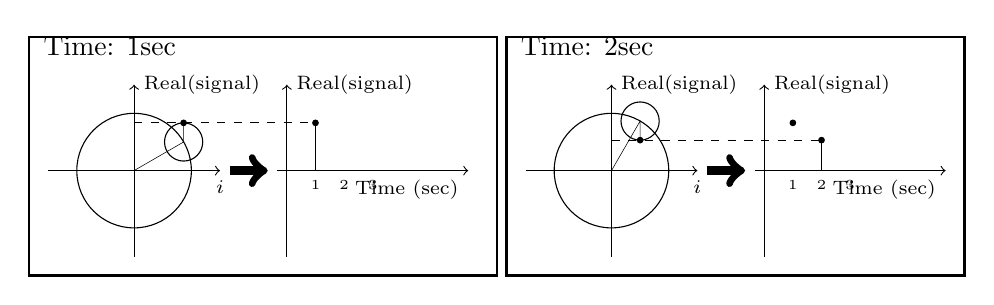
\begin{tikzpicture}

  %% Border rectangle and label.
  \draw [line width=1pt] (0,0)
  rectangle (0.49\linewidth, 0.25\linewidth);
  \draw [anchor=south west] (0.005\linewidth, 0.22\linewidth)
  node {Time: 1sec};

  %% The main imaginary axises:
  \draw[->] (0.02\linewidth, 0.11\linewidth)
  -- (0.2\linewidth, 0.11\linewidth);
  \draw[anchor=north] (0.2\linewidth, 0.11\linewidth)
  node {\scriptsize $i$};
  \draw[->] (0.11\linewidth, 0.02\linewidth)
  -- (0.11\linewidth, 0.20\linewidth);
  \draw[anchor=west] (0.11\linewidth, 0.20\linewidth)
  node {\scriptsize Real(signal)};

  %% The circles
  \draw (0.11\linewidth,0.11\linewidth) circle [radius=0.06\linewidth];
  \draw (0.1619\linewidth,0.14\linewidth) circle [radius=0.02\linewidth];
  \draw[very thin] (0.11\linewidth, 0.11\linewidth)
  -- (0.1619\linewidth,0.14\linewidth)
  -- (0.1619\linewidth,0.16\linewidth);
  \draw[fill=black] (0.1619\linewidth,0.16\linewidth) circle [radius=1pt];


  %% The connections:
  \draw[->, line width=3pt] (0.21\linewidth, 0.11\linewidth)
  -- (0.25\linewidth, 0.11\linewidth);
  \draw[dashed, thin] (0.11\linewidth,0.16\linewidth)
  -- (0.30\linewidth,0.16\linewidth);


  %% The signal vs. time axises:
  \draw[->] (0.26\linewidth, 0.11\linewidth)
  -- (0.46\linewidth, 0.11\linewidth);
  \draw[anchor=north east] (0.46\linewidth, 0.11\linewidth)
  node {\scriptsize Time (sec)};
  \draw[->] (0.27\linewidth, 0.02\linewidth)
  -- (0.27\linewidth, 0.20\linewidth);
  \draw[anchor=west] (0.27\linewidth, 0.20\linewidth)
  node {\scriptsize Real(signal)};


  %% The point in the signal vs. time axis:
  \draw[fill=black] (0.30\linewidth,0.16\linewidth) circle [radius=1pt];
  \draw[thin] (0.30\linewidth, 0.11\linewidth)
  -- (0.30\linewidth, 0.16\linewidth);
  \draw[anchor=north] (0.30\linewidth, 0.11\linewidth) node {\tiny 1};
  \draw[anchor=north] (0.33\linewidth, 0.11\linewidth) node {\tiny 2};
  \draw[anchor=north] (0.36\linewidth, 0.11\linewidth) node {\tiny 3};

















  \draw [line width=1pt] (0.5\linewidth,0)
  rectangle (0.98\linewidth, 0.25\linewidth);
  \draw [anchor=south west] (0.505\linewidth, 0.22\linewidth)
  node {Time: 2sec};


  %% The main imaginary axises:
  \draw[->] (0.52\linewidth, 0.11\linewidth)
  -- (0.7\linewidth, 0.11\linewidth);
  \draw[anchor=north] (0.7\linewidth, 0.11\linewidth)
  node {\scriptsize $i$};
  \draw[->] (0.61\linewidth, 0.02\linewidth)
  -- (0.61\linewidth, 0.20\linewidth);
  \draw[anchor=west] (0.61\linewidth, 0.20\linewidth)
  node {\scriptsize Real(signal)};

  %% The circles
  \draw (0.61\linewidth,0.11\linewidth) circle [radius=0.06\linewidth];
  \draw (0.64\linewidth,0.1619\linewidth) circle [radius=0.02\linewidth];
  \draw[very thin] (0.61\linewidth, 0.11\linewidth)
  -- (0.64\linewidth,0.1619\linewidth)
  -- (0.64\linewidth,0.1419\linewidth);
  \draw[fill=black] (0.64\linewidth,0.1419\linewidth) circle [radius=1pt];


  %% The connections:
  \draw[->, line width=3pt] (0.71\linewidth, 0.11\linewidth)
  -- (0.75\linewidth, 0.11\linewidth);
  \draw[dashed, thin] (0.61\linewidth,0.1419\linewidth)
  -- (0.83\linewidth,0.1419\linewidth);


  %% The signal vs. time axises:
  \draw[->] (0.76\linewidth, 0.11\linewidth)
  -- (0.96\linewidth, 0.11\linewidth);
  \draw[anchor=north east] (0.96\linewidth, 0.11\linewidth)
  node {\scriptsize Time (sec)};
  \draw[->] (0.77\linewidth, 0.02\linewidth)
  -- (0.77\linewidth, 0.20\linewidth);
  \draw[anchor=west] (0.77\linewidth, 0.20\linewidth)
  node {\scriptsize Real(signal)};


  %% The point in the signal vs. time axis:
  \draw[fill=black] (0.80\linewidth,0.16\linewidth) circle [radius=1pt];
  \draw[fill=black] (0.83\linewidth,0.1419\linewidth) circle [radius=1pt];
  \draw[thin] (0.83\linewidth, 0.11\linewidth)
  -- (0.83\linewidth, 0.1419\linewidth);
  \draw[anchor=north] (0.80\linewidth, 0.11\linewidth) node {\tiny 1};
  \draw[anchor=north] (0.83\linewidth, 0.11\linewidth) node {\tiny 2};
  \draw[anchor=north] (0.86\linewidth, 0.11\linewidth) node {\tiny 3};

\end{tikzpicture}


% This TeX document is part of the manual of the GNU Astronomy
% Utilities (Gnuastro). A Makefile is also distributed which allows
% you to compile this TeX file in the desired manner.
%
% Original author:
%     Mohammad Akhlaghi <mohammad@akhlaghi.org>
% Contributing author(s):
% Copyright (C) 2015-2018, Free Software Foundation, Inc.
%
% Gnuastro is free software: you can redistribute it and/or modify it
% under the terms of the GNU General Public License as published by
% the Free Software Foundation, either version 3 of the License, or
% (at your option) any later version.
%
% Gnuastro is distributed in the hope that it will be useful, but
% WITHOUT ANY WARRANTY; without even the implied warranty of
% MERCHANTABILITY or FITNESS FOR A PARTICULAR PURPOSE.  See the GNU
% General Public License for more details.
%
% You should have received a copy of the GNU General Public License
% along with Gnuastro. If not, see <http://www.gnu.org/licenses/>.

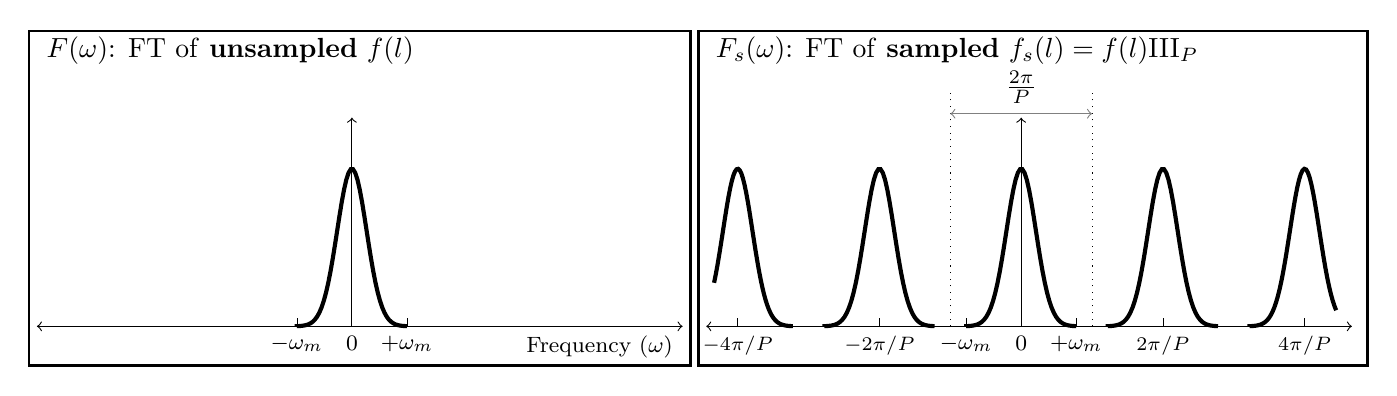
\begin{tikzpicture}[samples=50]

  %% Border rectangle and label.
  \draw [line width=1pt] (0,0) rectangle (8.4cm, 4.25cm);
  \draw [anchor=south west] (0.1cm, 3.7cm)
  node {$F(\omega)$: FT of \textbf{unsampled} $f(l)$};


  %% Draw the axis:
  \draw[<->] (0.1cm, 0.5cm) -- (8.3cm, 0.5cm);
  \draw[anchor=north east] (8.3cm, 0.5cm) node {\footnotesize Frequency ($\omega$)};
  \draw[->] (4.1cm, 0.5cm) -- (4.1cm, 3.15cm);


  %% Draw the main plot
  \draw[line width=1.5pt, domain=3.4:4.8]
  (3.4,0.5) -- plot (\x, {2*exp(-((\x-4.1)^2)/0.07)+0.5});
  \draw[very thin, anchor=north] (3.4,0.6) -- (3.4,0.5)
  node {\footnotesize $-\omega_m$};
  \draw[very thin, anchor=north] (4.8,0.6) -- (4.8,0.5)
  node {\footnotesize $+\omega_m$};
  \draw[anchor=north] (4.1,0.5) node {\footnotesize $0$};








  %% Border rectangle and label.
  \draw [line width=1pt] (8.5cm,0) rectangle (17cm, 4.25cm);
  \draw [anchor=south west] (8.6cm, 3.7cm)
  node {$F_s(\omega)$: FT of \textbf{sampled} $f_s(l)=f(l)\mathrm{III}_P$};


  %% Draw the axis:
  \draw[<->] (8.6cm, 0.5cm) -- (16.8cm, 0.5cm);
  \draw[->] (12.6cm, 0.5cm) -- (12.6cm, 3.15cm);


  %% Draw the main plot
  \draw[line width=1.5pt, domain=11.9:13.3]
  (11.9,0.5) -- plot (\x, {2*exp(-((\x-12.6)^2)/0.07)+0.5});
  \draw[very thin, anchor=north] (11.9,0.6) -- (11.9,0.5)
  node {\footnotesize $-\omega_m$};
  \draw[very thin, anchor=north] (13.3,0.6) -- (13.3,0.5)
  node {\footnotesize $+\omega_m$};
  \draw[anchor=north] (12.6,0.5) node {\footnotesize $0$};


  %% Draw the region:
  \draw[anchor=east, dotted] (11.7,0.5) -- (11.7,3.5);
  \draw[anchor=west, dotted] (13.5,0.5) -- (13.5,3.5);
  \draw[<->, color=gray, thin] (11.7,3.2) -- (13.5,3.2);
  \draw[anchor=south] (12.6,3.2) node {$\frac{2{\pi}}{P}$};


  %% Next plot (first positive)
  \draw[line width=1.5pt, domain=13.7:15.1]
  (13.7,0.5) -- plot (\x, {2*exp(-((\x-14.4)^2)/0.07)+0.5});
  \draw[very thin, anchor=north]
  (14.4,0.6) -- (14.4,0.5) node {\scriptsize $2{\pi}/P$};

  %% Next plot (second positive)
  \draw[line width=1.5pt, domain=15.5:16.6]
  (15.5,0.5) -- plot (\x, {2*exp(-((\x-16.2)^2)/0.07)+0.5});
  \draw[very thin, anchor=north]
  (16.2,0.6) -- (16.2,0.5) node {\scriptsize $4{\pi}/P$};

  %% Next plot (first negative)
  \draw[line width=1.5pt, domain=10.1:11.5]
  (10.1,0.5) -- plot (\x, {2*exp(-((\x-10.8)^2)/0.07)+0.5});
  \draw[very thin, anchor=north]
  (10.8,0.6) -- (10.8,0.5) node {\scriptsize $-2{\pi}/P$};

  %% Next plot (second negative)
  \draw[line width=1.5pt, domain=8.7:9.7]
  plot (\x, {2*exp(-((\x-9)^2)/0.07)+0.5});
  \draw[very thin, anchor=north]
  (9,0.6) -- (9,0.5) node {\scriptsize $-4{\pi}/P$};

\end{tikzpicture}


% This TeX document is part of the manual of the GNU Astronomy
% Utilities (Gnuastro). A Makefile is also distributed which allows
% you to compile this TeX file in the desired manner.
%
% Original author:
%     Mohammad Akhlaghi <mohammad@akhlaghi.org>
% Contributing author(s):
% Copyright (C) 2016-2021, Free Software Foundation, Inc.
%
% Gnuastro is free software: you can redistribute it and/or modify it
% under the terms of the GNU General Public License as published by
% the Free Software Foundation, either version 3 of the License, or
% (at your option) any later version.
%
% Gnuastro is distributed in the hope that it will be useful, but
% WITHOUT ANY WARRANTY; without even the implied warranty of
% MERCHANTABILITY or FITNESS FOR A PARTICULAR PURPOSE.  See the GNU
% General Public License for more details.
%
% You should have received a copy of the GNU General Public License
% along with Gnuastro. If not, see <http://www.gnu.org/licenses/>.

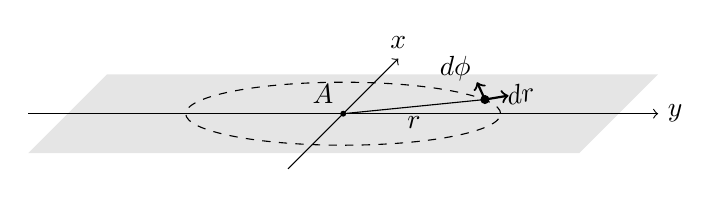
\begin{tikzpicture}

  \fill[fill=black!10!white]
  (-2.5,0.5) -- ++(7,0) -- ++(-1,-1) -- ++(-7,0) -- cycle;

  \filldraw (0.5,0) circle (0.03);
  \draw (0.5,0) node[anchor=south east]{$A$};
  \draw[dashed] (0.5,0) ellipse (2 and 0.4);
  \draw (0.5,0) -- node[anchor=north]{$r$}(2.3,0.18);
  \filldraw (2.3,0.18) circle (0.05);
  \draw[->, thick]
  (2.3,0.18) -- node[anchor=west, rotate=10]{$dr$}(2.6,0.23);
  \draw[->, thick]
  (2.3,0.18) -- node[anchor=south east]{$d\phi$}(2.2,0.4);
  \draw[<-, thin] (1.2,0.7) -- (-0.2,-0.7); %along y=x-0.5
  \draw[->, thin] (-3.5,0) -- (4.5,0);
  \draw (1.2,0.7) node[anchor=south]{$x$};
  \draw (4.5,0) node[anchor=west]{$y$};

\end{tikzpicture}


% This TeX document is part of the manual of the GNU Astronomy
% Utilities (Gnuastro). A Makefile is also distributed which allows
% you to compile this TeX file in the desired manner.
%
% Original author:
%     Mohammad Akhlaghi <mohammad@akhlaghi.org>
% Contributing author(s):
% Copyright (C) 2016-2019, Free Software Foundation, Inc.
%
% Gnuastro is free software: you can redistribute it and/or modify it
% under the terms of the GNU General Public License as published by
% the Free Software Foundation, either version 3 of the License, or
% (at your option) any later version.
%
% Gnuastro is distributed in the hope that it will be useful, but
% WITHOUT ANY WARRANTY; without even the implied warranty of
% MERCHANTABILITY or FITNESS FOR A PARTICULAR PURPOSE.  See the GNU
% General Public License for more details.
%
% You should have received a copy of the GNU General Public License
% along with Gnuastro. If not, see <http://www.gnu.org/licenses/>.

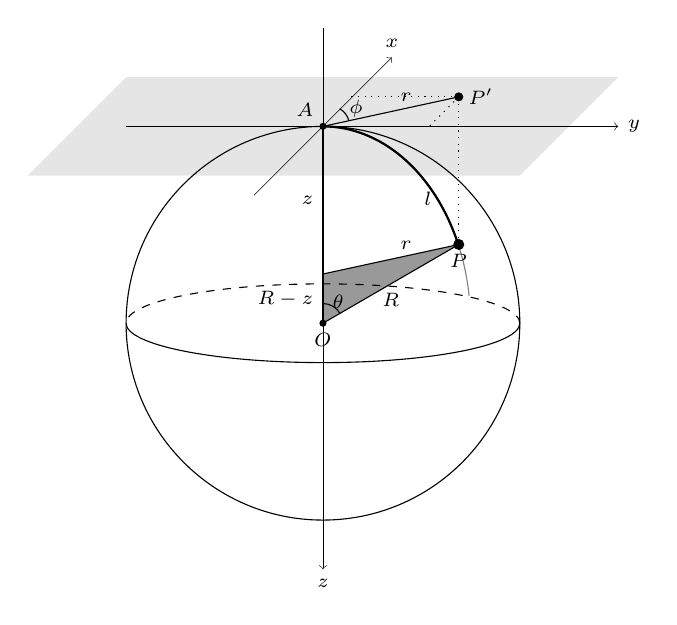
\begin{tikzpicture}[scale=1.25]
  \tikzstyle{every node}=[font=\scriptsize]
  %parallelogram: 2D surface
  \fill[fill=black!10!white]
  (-1.5,0.5) -- ++(5,0) -- ++(-1,-1) -- ++(-5,0) -- cycle;

  %Triangle:
  \filldraw[fill=black!40!white, draw=black]
  (0.5,-2) -- node[anchor=north]{$R$}(1.88,-1.2)
  -- node[anchor=south west]{$r$}(0.5, -1.5) -- cycle;
  \draw (0.5,-1.8) arc (90:30:0.2);
  \draw (0.5,0) -- node[anchor=east]{$z$}(0.5,-1.5)
  -- node[anchor=east]{$R-z$}(0.5,-2);
  \draw (0.5,-1.95) node[anchor=south west]{$\theta$};

  %Cartesian Coordinates, sphere and their names
  \draw[<-, very thin] (1.2,0.7) -- (-0.2,-0.7);
  \draw (1.2,0.7) node[anchor=south]{$x$};

  \draw[->, very thin] (-1.5,0) -- (3.5,0);
  \draw (3.5,0) node[anchor=west]{$y$};

  \draw[->, very thin] (0.5,1) -- (0.5,-4.5);
  \draw (0.5,-4.5) node[anchor=north]{$z$};

  \draw (0.5,-2) circle (2);
  \draw (-1.5,-2) arc (180:360:2 and 0.4);
  \draw[dashed] (2.5,-2) arc (0:180:2 and 0.4);

  \filldraw (0.5,0) circle (0.03);
  \draw (0.5,0) node[anchor=south east]{$A$};

  \filldraw (0.5,-2) circle (0.03);
  \draw (0.5,-2) node[anchor=north]{$O$};

  \draw (0.67,0.18) arc (60:15:0.2);
  \draw (0.67,0.18) node[anchor=west]{$\phi$};

  %P and it's arcs
  \draw[thin, gray] (0.5,0) arc(90:8:1.5 and 2);
  \draw[thick] (0.5,0) arc(90:25:1.5 and 2);

  \filldraw (1.88,-1.2) circle (0.05);
  \draw (1.88,-1.2) node[anchor=north]{$P$};
  \filldraw (1.88,0.3) circle (0.04);
  \draw[dotted] (1.88,-1.2) -- (1.88, 0.3);

  %Images of P and P' on 2D plane:
  \draw (1.88,0.3) node[anchor=west]{$P'$};
  \draw (0.5,0) -- node[anchor=south west]{$r$}(1.88, 0.3);
  \draw[dotted] (1.88,0.3) -- ++(-1.1,0);
  \draw[dotted] (1.88,0.3) -- ++(-0.3,-0.3);

  % Label chi:
  \draw (1.43, -0.9) node[anchor=south west]{$l$};
\end{tikzpicture}


\end{document}
